\chapter{*タイトル*}
\label{*Ltitle*}

タイトルの中身だよ。

\subsection{サブセクション}
\label{*Lsubsection*}

サブセクション\cite{*AuthorName*}の中身だよ。\figref{test} %画像番号。(Fig1.1)など



\begin{itemize}
\item アイテム1
\item アイテム2
\item アイテム3。文章に出来るよ
\end{itemize}

\begin{figure}[h]
  \centering
  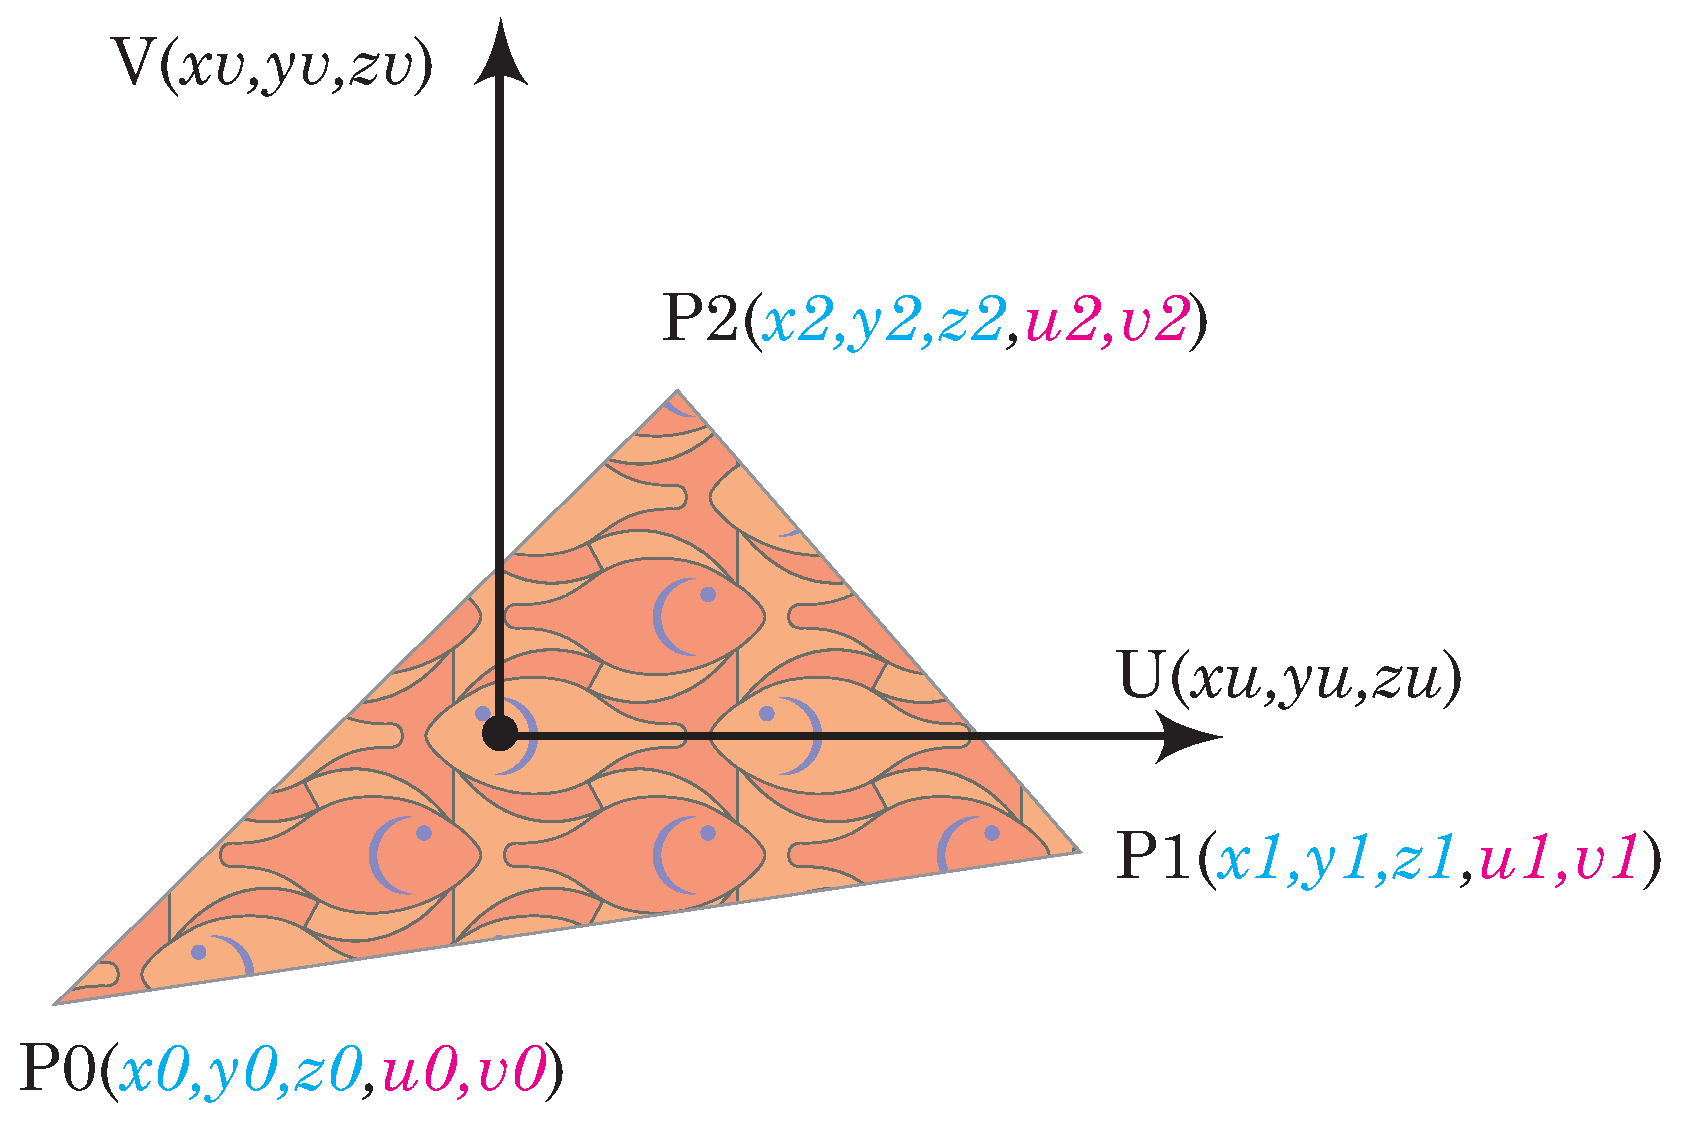
\includegraphics[width=3.0in]{./img/polygon_explain}
  \caption{キャプションだよ}{行を変えられるみたい}
  \label{test} %ここで画像のラベリング?
\end{figure}
 
